\documentclass[main.tex]{subfiles}
% 函数的极限与连续性
\begin{document}
我们用“$\varepsilon-\delta$语言”来定义函数极限。

\begin{definition}[向量函数的极限]\label{def:II.4.5}
    给定函数$\mathbf{f}:\mathbb{R}^n\supset D\rightarrow\mathbb{R}^m$,如果对任意正实数$\varepsilon$总存在正实数$\delta$使得只要$0<\left\|\mathbf{r}-\mathbf{r}_0\right\|<\delta,\mathbf{r},\mathbf{r}_0\in D$,就总有$\left\|\mathbf{f}\left(\mathbf{r}\right)-\mathbf{y}_0\right\|<\varepsilon,\mathbf{y}_0\in\mathbb{R}^m$,就称$\mathbf{y}_0$是函数$\mathbf{f}\left(\mathbf{r}\right)$在$\mathbf{r}_0$处的\emph{极限(limit)},记为
    \[\lim_{\mathbf{r} \to\mathbf{r}_0} \mathbf{f}\left(\mathbf{r}\right)=\mathbf{y}_0\]
\end{definition}

\begin{theorem}\label{thm:II.4.1}
    函数$\mathbf{f}:\mathbb{R}^n\supset D\rightarrow\mathbb{R}^m$在$\mathbf{r}_0\in D$处存在极限$\lim_{\mathbf{r}\to\mathbf{r}_0}\mathbf{f}\left(\mathbf{r}\right)=\mathbf{a},\mathbf{a}=\left(a_i\right)\in\mathbb{R}^m$的充要条件是其坐标函数的极限$\lim_{\mathbf{r}\to\mathbf{r}_0}f_i\left(\mathbf{r}\right)=a_i,\forall i=1,\cdots,m$都存在。
\end{theorem}
\begin{proof}
    由向量函数定义,$\mathbf{f}$与$f_i,i=1,\cdots,m$的定义域都相同。

    若已知$\lim_{\mathbf{r}\to\mathbf{r}_0}\mathbf{f}\left(\mathbf{r}\right)=\mathbf{a}$,即对任一实数$\varepsilon>0$都存在实数$\delta>0$使得只要$0<\left\|\mathbf{r}-\mathbf{r}_0\right\|<\delta$就有$\left\|\mathbf{f}\left(\mathbf{r}\right)-\mathbf{a}\right\|<\varepsilon$。那么,取同一对正实数$\varepsilon$和$\delta$,对任一$i\in\left\{1,\cdots,m\right\}$都有
    \begin{align*}
        \left|f_i\left(\mathbf{r}\right)-\alpha_i\right| & \leq\sum_{i=1}^m\left|f_i\left(\mathbf{r}\right)-a_i\right|\quad\text{(当}m=1\text{或}f_j=a_j\forall j\neq i\text{时取等号。)} \\
                                                         & \leq\left|\sum_{i=1}^m\left(f_i\left(\mathbf{r}\right)-\alpha_i\right)\right|\quad\text{(三角不等式。)}                       \\
                                                         & =\left\|\mathbf{f}\left(\mathbf{r}\right)-\mathbf{a}\right\|<\varepsilon
    \end{align*}
    故按照极限的定义,$\lim_{\mathbf{r}\to\mathbf{r}_0}f_i\left(\mathbf{r}\right)=\alpha_i,i=1,\cdots,m$,其中$a_i,i=1,\cdots,n$是$\mathbf{a}$的坐标。

    反之,若极限$\lim_{\mathbf{r}\to\mathbf{r}_0}f_i\left(\mathbf{r}\right)=a_i,i=1,\cdots,m$都存在,即对任一实数$\varepsilon>0$都能找到实数$\delta_i>0,i=1,\cdots,m$,使得只要$f_i$的定义域$D$内一向量$\mathbf{r}$到$\mathbf{r}_0$的距离满足$0<\left\|\mathbf{r}-\mathbf{r}_0\right\|<\delta_i$,就有$\left|f_i\left(\mathbf{r}\right)-a_i\right|<\varepsilon/\sqrt{m}$,那么令$\delta=\mathrm{min}\left\{\delta_1,\cdots,\delta_m\right\}$,则当$0<\left\|\mathbf{r}-\mathbf{r}_0\right\|<\delta$,就有$\mathrm{max}\left\{\left|f_i\left(\mathbf{r}\right)-a_i\right|\right\}<\varepsilon/\sqrt{m}$。

    利用事实\footnote{
        由$\left\|\mathbf{x}\right\|^2=\sum_{i=1}^nx_i^2\leq n\mathrm{max}\left\{x_1^2,\cdots,x_n^2\right\}$得到。
    }
    \[\left\|\mathbf{x}\right\|\leq\sqrt{n}\mathrm{max}\left\{\left|x_1\right|,\cdots,\left|x_n\right|\right\},\forall\mathbf{x}\in\mathbb{R}^n\]
    可得
    \[\left\|\mathbf{f}\left(\mathbf{r}\right)-\mathbf{a}\right\|\leq\sqrt{m}\mathrm{max}\left\{\left|f_i\left(\mathbf{r}\right)-a_i\right|\right\}<\varepsilon\]
    这样的$\delta$是总能取到的,故由函数极限的定义,$\lim_{\mathbf{r}\to\mathbf{r}_0}\mathbf{f}\left(\mathbf{r}\right)=\mathbf{a}$。
\end{proof}

定义\ref{def:II.4.5}表示,若$\lim_{\mathbf{x}\to\mathbf{x}_0}\mathbf{f}\left(\mathbf{x}\right)=\mathbf{y}_0$,则只要点$\mathbf{x}\neq\mathbf{x}_0$足够靠近$\mathbf{x}_0$,则$\mathbf{f}\left(\mathbf{x}\right)$总可以任意近地靠近点$\mathbf{y}_0$,而且$\mathbf{f}\left(\mathbf{x}_0\right)$未必等于$\mathbf{y}_0$。结合\S\ref{sec:B.1}定义的概念,点$\mathbf{r}_0$是$\mathrm{dom}\mathbf{f}$中的一个极限点,$0<\left\|\mathbf{r}-\mathbf{r}_0\right\|<\delta$是点$\mathbf{r}_0$的一个去心邻域。若$\lim_{\mathbf{x}\to\mathbf{x}_0}\mathbf{f}\left(\mathbf{x}\right)=\mathbf{y}_0$,则对$\mathbf{y}_0$的任一邻域$B_\varepsilon\left(\mathbf{y}_0\right)\subset\mathbb{R}^m$,总存在点$\mathbf{x}_0$的邻域$B_\delta\left(\mathbf{x}_0\right)\subset \mathbf{R}^n$,使得集合$B_\delta\left(\mathbf{x}_0\right)\cup D$在$\mathbf{f}$下的像集是$B_\varepsilon\left(\mathbf{y}_0\right)$的子集(如图\ref{fig:II.4.6})。

\begin{figure}[h]
    \centering
    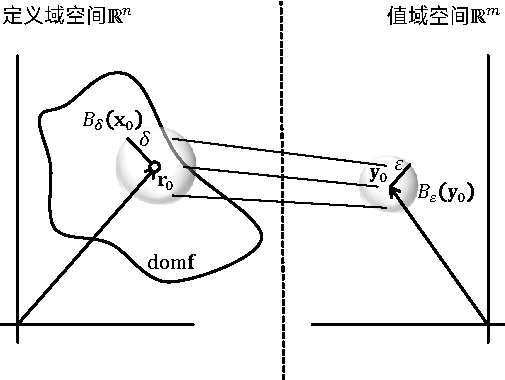
\includegraphics[width=0.75\textwidth]{images/II.4.6.pdf}
    \caption{向量函数的极限(定义\ref{def:II.4.5})的图像化理解。}
    \label{fig:II.4.6}
\end{figure}

\begin{definition}[函数的连续性]\label{def:II.4.6}
    给定函数$\mathbf{f}:\mathbb{R}^n\supset D\rightarrow\mathbb{R}^m$和其定义域中一点$\mathbf{r}_0\in D$。如果极限$\lim_{\mathbf{r}\to\mathbf{r}_0}\mathbf{f}\left(\mathbf{r}\right)=\mathbf{f}\left(\mathbf{r}_0\right)$存在,则称$\mathbf{f}\left(\mathbf{r}\right)$\emph{在$\mathbf{r}_0$处连续(continuous at $\mathbf{r}_0$)}。
\end{definition}

\begin{theorem}\label{thm:II.4.2}
    函数$\mathbf{f}:\mathbb{R}^n\supset D\rightarrow\mathbb{R}^m$在$\mathbf{r}_0\in D$处连续的充要条件是$\mathbf{f}$的坐标函数在$\mathbf{r}_0$处都连续。
\end{theorem}
\begin{proof}
    由定理\ref{thm:II.4.1}直接得证。
\end{proof}

如果一个函数$\mathbf{f}$在其定义域$D$内处处都连续,我们就直接称函数$\mathbf{f}$\emph{在$D$内连续(continuous in $D$)},或称函数$\mathbf{f}$是\emph{$D$上的连续函数(continuous function on $D$)}。以下给出的定理及其推论告诉我们:\emph{线性变换总是连续的}。

\begin{theorem}\label{thm:II.4.3}
    设$\mathcal{V}$、$\mathcal{W}$分别是数域$\mathbb{F}$上的$n,m$维赋范向量空间,$\mathbf{L}:\mathcal{V}\rightarrow\mathcal{W}$是一个线性变换,则总存在正实数$k>0$使得$\left\|\mathbf{Lx}\right\|\leq k\left\|\mathbf{x}\right\|,\forall\mathbf{x}\in\mathcal{V}$,当且仅当$n=1$时取等号。
\end{theorem}
\begin{proof}
    设$\left\{\mathbf{e}_i\right\}$是$\mathcal{V}$的一组基,则任一向量$\mathbf{x}\in\mathcal{V}$可表示为$\mathbf{x}=\sum_{i=1}^nx_i\mathbf{e}_i$。设$\left\|\cdot\right\|_\mathrm{E}$是欧几里得范,即$\left\|\mathbf{x}\right\|_\mathrm{E}\equiv\left(\sum_{i=1}^nx_i^2\right)^\frac{1}{2}$。由定理\ref{thm:II.2.23}及其推论,包括欧几里得范在内的任意范都不依赖基的选择。故在任一基下总有$\left|x_i\right|\leq\left(\sum_{i=1}^nx_i^2\right)^\frac{1}{2}=\left\|\mathbf{x}\right\|_\mathrm{E}$。

    由引理\ref{lem:A.1},对$\mathcal{V}$上的任一范的定义$\left\|\cdot\right\|$,总存在$K>0$使得$\left\|\cdot\right\|_\mathrm{E}\leq K\left\|\cdot\right\|$。故
    \begin{align*}
        \left\|\mathbf{Lx}\right\| & =\left\|\sum_{i=1}^nx_i\mathbf{Le}_i\right\|                                                     \\
                                   & \leq\sum_{i=1}^n\left|x_i\right|\left\|\mathbf{Le}_i\right\|                                     \\
                                   & \leq\sum_{i=1}^n\left\|\mathbf{x}\right\|_\mathrm{E}\left\|\mathbf{Le}_i\right\|                 \\
                                   & \leq\sum_{i=1} K\left\|\mathbf{x}\right\|\left\|\mathbf{Le}_i\right\|=k\left\|\mathbf{x}\right\|
    \end{align*}
    其中$k=K\sum_{i=1}^n\left\|\mathbf{Le}_i\right\|$。上面的第2个不等号用到范的三角不等式和范的调和性,第三个不等号用到证明开头提到的事实,第四个不等号用到引理\ref{lem:A.1}。由于引理\ref{lem:A.1}的等号当且仅当$n=1$时成立,这一条件已经强于其余两个不等号的取等充要条件,故整个不等式的取等充要条件就是$n=1$。
\end{proof}

\begin{corollary}
    线性变换是连续函数。
\end{corollary}
\begin{proof}
    由定理\ref{thm:II.4.3},对任意$\mathbf{x},\mathbf{x}_0\in\mathcal{V}$有$\left\|\mathbf{Lx}-\mathbf{Lx}_0\right\|=\left\|\mathbf{L}\left(\mathbf{x}-\mathbf{x}_0\right)\right\|\leq k\left\|\mathbf{x}-\mathbf{x}_0\right\|$,故对任一$\varepsilon>0$总可取$\delta=\frac{\varepsilon}{k}$使得只要$\left\|\mathbf{x}-\mathbf{x}_0\right\|<\delta$就有$\left\|\mathbf{Lx}-\mathbf{Lx}_0\right\|\leq k\left\|\mathbf{x}-\mathbf{x}_0\right\|<k\delta=\varepsilon$。
\end{proof}

由定理\ref{thm:II.4.1}和\ref{thm:II.4.2},向量函数的极限存在性和连续性总可以通过其坐标函数的极限存在性和连续性得到证明,使得问题回到本科高等数学课的范围内。以下函数极限的性质,也已在本科的高等数学课中教过了,在此列出而不作证明。
\begin{theorem}[函数极限的基本性质]\label{thm:II.4.4}
    在实数域内,以下命题成立:
    \begin{enumerate}
        \item 设$a,b$是常数,则$\lim_{x\to a}b=b$。
        \item 若$a$是常数,则$\lim_{x\to a} x=a$。
        \item 设$\lim_{x\to a}f\left(x\right)=L$,$c$是常数,则$\lim_{x\to a}cf\left(x\right)=c\lim_{x\to a}f\left(x\right)=cL$。
        \item 设$\lim_{x\to c}f\left(x\right)=L,\lim_{x\to c}g\left(x\right)=M$,则$\lim_{x\to c}\left[f\left(x\right)+g\left(x\right)\right]=L+M$。
        \item 设$\lim_{x\to c}f\left(x\right)=L,\lim_{x\to c}g\left(x\right)=M$,则$\lim_{x\to c}\left[f\left(x\right)g\left(x\right)\right]=LM$。
        \item (夹逼定理)若$c$是常数,$g\left(x\right)\leq f\left(x\right)\leq h\left(x\right)$至少在点$x=c$之外都成立,且$\lim_{x\to c}g\left(x\right)=\lim_{x\to c}h\left(x\right)=L$,则$\lim_{x\to c}f\left(x\right)=L$。
        \item 设$\lim_{x\to c}f\left(x\right)=L$,则$\left|\lim_{x\to c}f\left(x\right)\right|=\left|L\right|=\lim_{x\to c}\left|f\left(x\right)\right|$。
    \end{enumerate}
\end{theorem}
\end{document}